\item \model{MobileLLM-Pro}

\paragraph*{سد محاسباتی آموزش بافت طولانی در مدل‌های ۱ میلیارد پارامتری}
مدل \model{MobileLLM-Pro} \cite{huber2025mobilellmpro} که جهت اجرای با تأخیر پایین بر روی دستگاه‌های موبایل با بافت ۱۲۸K توکن طراحی شده، ساختار توجه محلی-سراسری (\en{Local-Global Attention}) به نسبت ۳ به ۱ با اندازه پنجره محلی ۵۱۲ توکن را به کار می‌گیرد. چالش اساسی این مدل در فاز آموزش متجلی می‌شود: آموزش مستقیم یک مدل کوچک روی بافت‌های ۱۲۸K مستلزم پردازش داده‌های طویل نادر است که به دلیل تغییر شدید توزیع داده نسبت به پیش‌آموزش عمومی اولیه ($L_{\text{short}} = 2048$)، منجر به افت محسوس ۵.۹ درصدی در بنچمارک‌های دانش عمومی می‌گردد.

\paragraph*{فرمول‌بندی تقطیر موقعیتی ضمنی (\en{Implicit Positional Distillation})}
برای حل این معضل، پژوهشگران متا سازوکار \textbf{تقطیر موقعیتی ضمنی} را معرفی کردند. در روش \en{RoPE}، بردار زاویه‌ای هر فرکانس در طول‌های کوتاه تنها زیرمجموعه محدودی از فضای زاویه‌ای قطبی را پوشش می‌دهد:
\begin{equation}
    \Delta \phi_j \in [0, \, \theta_j \cdot L_{\text{short}}], \quad \theta_j = 10000^{-2(j-1)/d}
\end{equation}
چسباندن اسناد کوتاه به یکدیگر به همراه ماسک علّی بلوکی نیز مشکل را حل نمی‌کند، زیرا روابط معنایی و گرادیان‌های یادگیری تنها در درون فواصل بسته هر سند منفرد ($\theta_{\max} - \theta_{\min} = \alpha$) محبوس مانده و مدل دانش‌آموز روابط زاویه‌ای در فواصل بزرگ را تجربه نمی‌کند. در رویکرد پیشنهادی، مدل دانش‌آموز روی همان توالی‌های کوتاه آموزش می‌بیند، اما هدف بهینه‌سازی آن کمینه‌سازی واگرایی کولبک-لایبلر با توزیع لاجیت‌های یک مدل معلم مقیاس‌بزرگ آموزش‌دیده در بافت‌های طویل (\en{Llama 4-Scout}) است:
\begin{equation}
    \mathcal{L}_{\text{KD}} = D_{\text{KL}}\left( P_{\text{teacher}}(y \mid x) \,\|\, P_{\text{student}}(y \mid x) \right) = \sum_{v \in \mathcal{V}} P_{\text{teacher}}(v \mid x) \log \left( \frac{P_{\text{teacher}}(v \mid x)}{P_{\text{student}}(v \mid x)} \right)
\end{equation}
از آنجا که توزیع لاجیت معلم روی دایره واژگان ۲۰۲,۰۴۸ توکنی به شکل ذاتی حاوی اطلاعات چگونگی تعامل توکن‌ها در سراسر فضای زاویه‌ای ۳۶۰ درجه RoPE است، مدل دانش‌آموز هندسه دوران و استدلال دوربرد را مستقیماً از احتمالات پیش‌بینی کلمات بعدی جذب می‌کند. نتایج نشان داد این رویکرد دقت بازیابی در آزمون «سوزن در انبار کاه» (\en{NIH}) را به ۹۹.۷۸٪ رسانده و افت کارایی در سایر بنچمارک‌ها را به کمتر از ۰.۲٪ تقلیل داده است.

\begin{latin}
\begin{center}
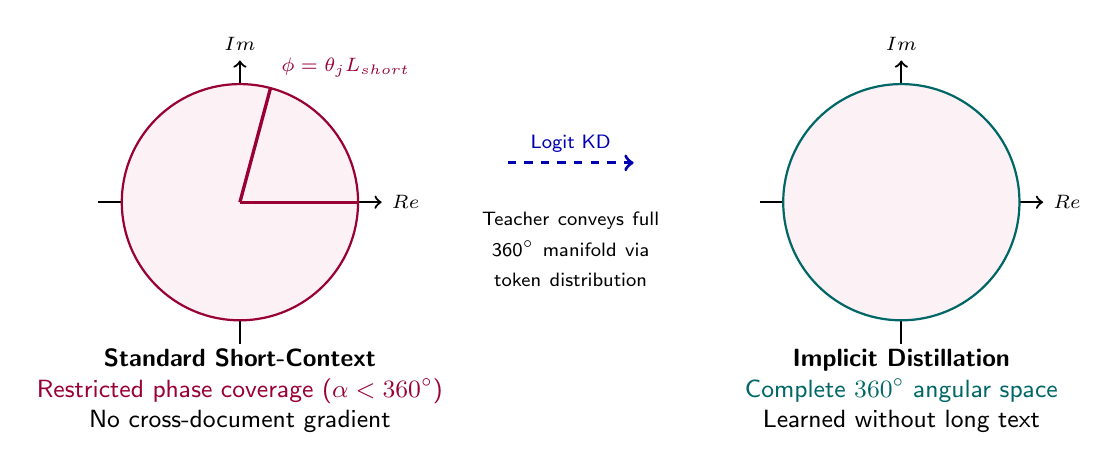
\begin{tikzpicture}[
    circ/.style={draw=purple!80!black, thick, fill=purple!5, circle, minimum size=3.2cm},
    sector_short/.style={fill=purple!35, draw=purple!80!black, thick},
    sector_full/.style={fill=teal!30, draw=teal!80!black, thick},
    label_node/.style={font=\small\sffamily, align=center}
]
    % Left: Short context limited angle
    \begin{scope}[shift={(0,0)}]
        \fill[purple!15] (0,0) -- (1.5,0) arc (0:75:1.5) -- cycle;
        \draw[thick, ->] (-1.8,0) -- (1.8,0) node[right] {\scriptsize $\text{Re}$};
        \draw[thick, ->] (0,-1.8) -- (0,1.8) node[above] {\scriptsize $\text{Im}$};
        \draw[circ] (0,0) circle (1.5cm);
        \draw[purple!80!black, very thick] (0,0) -- (75:1.5) node[above right] {\scriptsize $\phi = \theta_j L_{\text{short}}$};
        \draw[purple!80!black, very thick] (0,0) -- (0:1.5);
        \node[label_node] at (0, -2.4) {\textbf{Standard Short-Context}\\\textcolor{purple!80!black}{Restricted phase coverage ($\alpha < 360^\circ$)}\\No cross-document gradient};
    \end{scope}

    % Middle: Teacher Logit Transfer
    \begin{scope}[shift={(4.2,0)}]
        \draw[->, very thick, dashed, color=blue!70!black] (-0.8, 0.5) -- (0.8, 0.5) 
            node[midway, above, font=\scriptsize\sffamily] {Logit KD};
        \node[label_node, text width=2.4cm] at (0, -0.6) {
            \scriptsize Teacher conveys full 360$^\circ$ manifold via token distribution
        };
    \end{scope}

    % Right: Full angle covered implicitly
    \begin{scope}[shift={(8.4,0)}]
        \fill[teal!25] (0,0) circle (1.5cm);
        \draw[thick, ->] (-1.8,0) -- (1.8,0) node[right] {\scriptsize $\text{Re}$};
        \draw[thick, ->] (0,-1.8) -- (0,1.8) node[above] {\scriptsize $\text{Im}$};
        \draw[circ, draw=teal!80!black] (0,0) circle (1.5cm);
        \node[label_node] at (0, -2.4) {\textbf{Implicit Distillation}\\\textcolor{teal!80!black}{Complete $360^\circ$ angular space}\\Learned without long text};
    \end{scope}
\end{tikzpicture}
\end{center}
\end{latin}